\section{Methodology}

%  \item background: CephFS implementation
To explore software-defined cache management, we use
the data management language and policy engine presented
in~\cite{sevilla:sc15-mantle}. The prototype in that paper was called Mantle
and it was originally built on the CephFS so administrators could control file
system metadata data management policies. We now refer to Mantle as a policy
engine that supports our data management language.  The basic premise is that
data management policies can be expressed with a simple API consisting of
``when", ``where", and ``how much". ``when" controls how aggressive or
conservative the decisions are; ``where" lets the policy control how
distributed or concentrated the data should be; and ``how much" controls the
amount of data that should be sent. There is also a ``load" policy that lets
administrators specify how to collapse many metrics into a single load metric
({\it e.g.}, \(2\times\texttt{cpu} + 3\times\texttt{memory usage}\)).

The succinctness of the API lets users inject multiple, possibly dynamic, policies. In
this work we focus on a single node, so the ``where" policy is not used. When
we move ParSplice to a distributed key-value store back-end, the ``where" policy
can be used determine which key-value pairs should be moved to which node.

\subsection{Extracting Mantle as a Library}
\label{sec:extracting}

%  \item motivation: Mochi load balancer microservice
%  \item library architecture, callbacks, environment

We extracted Mantle as a library and Figure~\ref{fig:mantle} shows how it is
linked into a service.  Administrators write policies from whatever domain they
choose ({e.g.}, statistics, machine learning, storage system) and the policies
are embedded into the runtime by Mantle. When the service makes decisions it
executes the administrator-defined policies for when/where/how much and returns
a decision.  To do this, the service needs to be modified to (1) provide an
environment of metrics and (2) identify where policies are set. These
modification points are shown by the colored boxes in Figure~\ref{fig:mantle}
and described below.

\begin{figure}[t]
  \noindent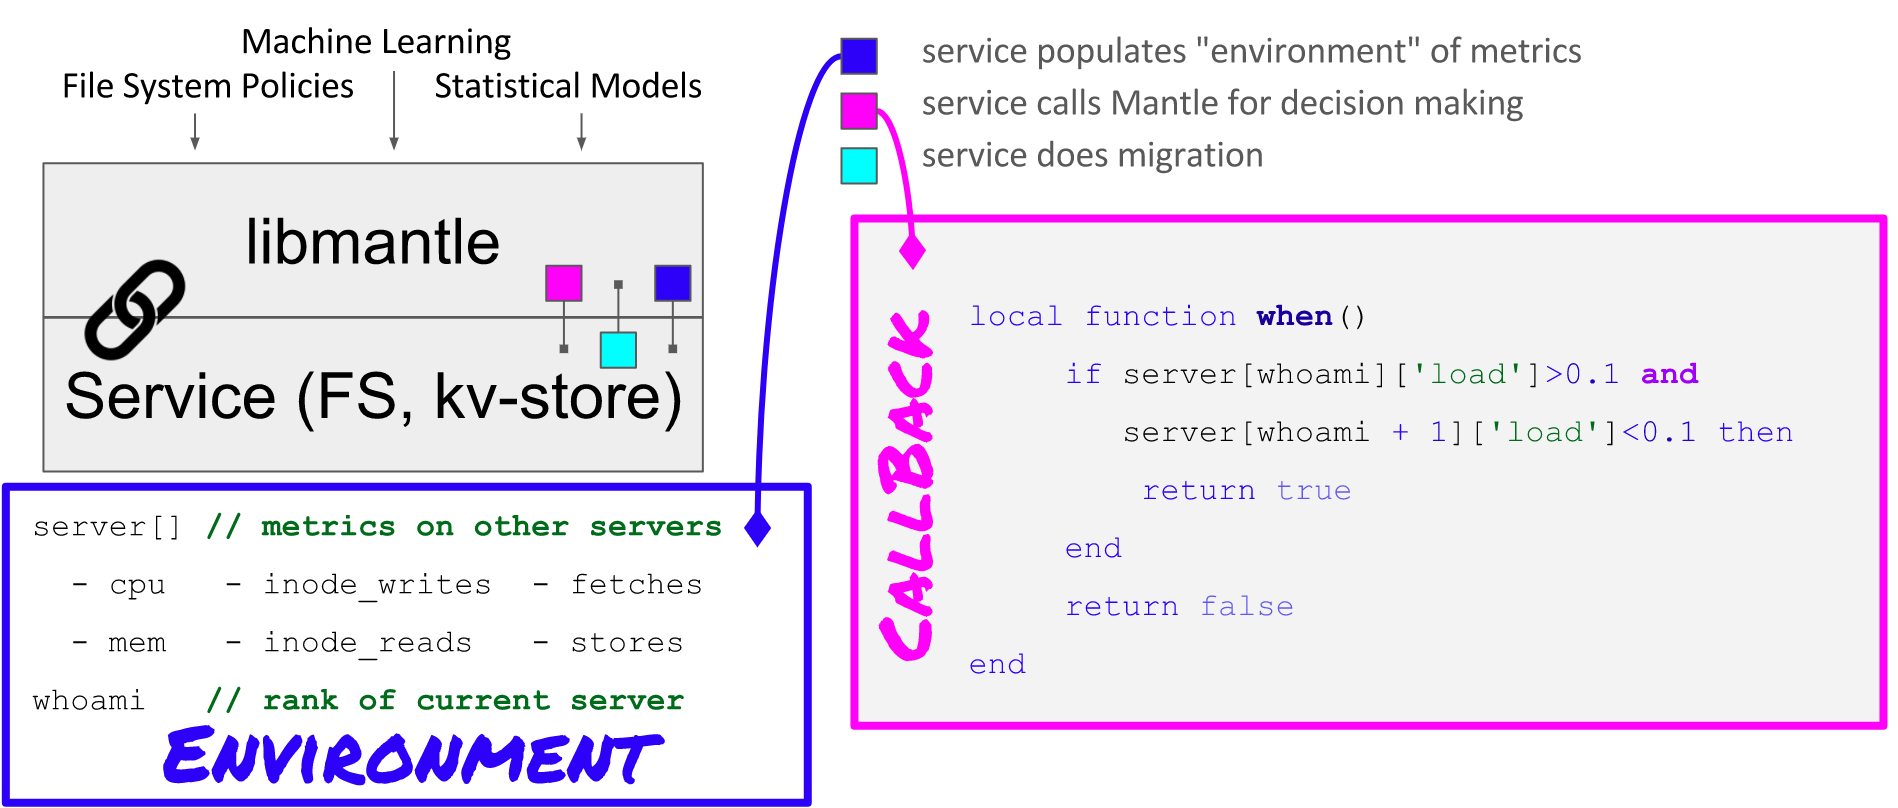
\includegraphics[width=0.5\textwidth]{figures/mantle.png}\\

  \caption{Extracting Mantle as library.\label{fig:mantle}}

\end{figure}

\begin{table}
  \centering
  \begin{tabular}{ r | l | l }
  Metrics     & Data Structure & Description \\\hline
  Cluster     & \{server \(\rightarrow\) \{metric \(\rightarrow\) val\}\}
              & resource util. for servers \\
  Time Series & [(ts, val), ..., (ts, val)]
              & accesses by timestamp (ts) \\
  && \\
              & Service      & Example \\\hline
  Cluster     & File Systems & CPU util., Inode reads \\
              & ParSplice    & CPU util., Cache size \\
  Time Series & File Systems & Accesses to directory \\
              & ParSplice    & Accesses to key in DB\\
  \end{tabular}
  \caption{Types of metrics exposed by the service to the policy engine using Mantle.\label{table:metrics}}
\end{table}

% policies themselves
\subsubsection{Policies Written as Callbacks} administrators write policies in
Lua that are executed whenever the service needs to make a data management
decision. We chose Lua for simplicity, performance, and portability; it is a
scripting language with simple syntax, which allows administrators to focus on
the policies themselves; it was designed as an embeddable language, so it is
lightweight and does less type checking; and it interfaces nicely with C/C++.
The ``callback" box in Figure~\ref{fig:mantle} shows an example policy for the
``when()" callback in a distributed service, where the current server
(\texttt{whoami}) migrates load if it is has load (\texttt{>0.1}) and if its
neighbor server (\texttt{whoami + 1}) does not have load (\texttt{<0.1}). The
load is calculated using the metrics provided by the environment.

Mantle also provides functions for persisting state across decisions.
\texttt{WRState(s)} saves state \texttt{s}, which can be a number or boolean
value, and \texttt{RDState()} returns the state saved by a previous iteration.
For example, a ``when" policy can avoid trimming a cache or migrating data if
it had performed that operation in the previous decision.

%\begin{figure}[h]
%\footnotesize
%\begin{minted}{lua}
%if RDState() == 1 then
%  WRState(0)   -- the next decision will return true
%  return false
%else then
%  WRState(1)   -- the next decision will return false
%  return true
%end
%\end{minted}
%\end{figure}

%of timestamp (ts), value pairs representing accesses over time types of
\subsubsection{Environment of Metrics} services can expose cluster metrics for
describing resource utilization and time series metrics for describing accesses
to some data structure over time. Table~\ref{table:metrics} shows how these
metrics are accessed from the policies written by administrators. 

For cluster metrics, the service passes a dictionary to Mantle, indexed by
server name and metric. Policies access the cluster metric values by indexing
into a Lua table using \texttt{server} and \texttt{metric}, where server is a
node identifier ({e.g.}, MPI Rank, metadata server name) and metric is a
resource name.  For example, a policy written for an MPI-based service can
access the CPU utilization of the first rank in a communication group using:

\begin{figure}[h]
\footnotesize
\begin{minted}{lua}
load = servers[0]['cpu']
\end{minted}
\end{figure}

Other examples metrics used for file system metadata load balancing are shown
by the ``environment" box in Figure~\ref{fig:mantle}. The measurements and
exchange of metrics between servers is done by the service; Mantle in CephFS
leverages metrics from other servers collected using CephFS's heartbeats.

For time series metrics, the service passes an array of \texttt{(timestamp,
value)} pairs to Mantle and the policies can iterate over the accesses. For
example, a policy that uses accesses to a directory in a file system as a
metric for load collects that information using:

\begin{figure}[h]
\footnotesize
\begin{minted}{lua}
ts = array()
for i=1,arraysize() do
  for time,value in string.gmatch(ts, (%w+=%w)) do
    if value == 'mydirectory' then
      count = count + 1
    end
  end
end
\end{minted}
\end{figure}

The service uses a pointer to the time series to facilitate time series with
many values, like accesses to a database or directory in the file system
namespace. This decision limits the time series metrics to only include values
from the {\it current } node, although this is not a limitation of Mantle
itself.

\subsection{Integrating Mantle into ParSplice}

% env of metrics
Using Mantle cluster metrics, we expose cache size, CPU utilization, and memory
pressure of the worker node to the cache management policies. In
Section~\S\ref{sec:parsplice-keyspace-analysis} we only end up using the cache
size although the other metrics proved to be valuable debugging tools. Using
Mantle time series metrics, we expose accesses to the cache as a list of
\texttt{timestamp, key id} pairs. In Section~\S\ref{sec:dom-specific}, we
explore a key access pattern detection algorithm that uses this metric.

% where policies are made
We link Mantle directly into the worker cache circled in red in
Figure~\ref{fig:parsplice}. We put the ``when" and ``how much" callbacks
alongside code that checks for memory pressure. It is executed right before the
worker processes incoming and outgoing put/get transactions to the cache. As
stated previously, we do not use the ``where" part of Mantle because we focus
on a single node, but this part of the API will be used when we move the caches
and storage nodes to a key-values store back-end that uses key load balancing and
repartitioning.
